\documentclass{article}
\usepackage{bm}
\usepackage{amssymb,amsmath}
\usepackage{color}
\usepackage{graphics}

\newcommand{\onehalf}{{\frac{1}{2}}}

\newcommand{\cH}{{\mathcal H}}
\newcommand{\cL}{{\mathcal L}}
\newcommand{\cM}{{\mathcal M}}

\newcommand{\bH}{\bm H}
\newcommand{\bP}{\bm B}
\newcommand{\bR}{\bm R}
\newcommand{\bB}{\bm B}
\newcommand{\Rinv}{{\bm R}^{-1}}
\newcommand{\bL}{\bm L}
\newcommand{\bM}{\bm M}

\newcommand{\xhat}{{\hat{x}}}
\newcommand{\yhat}{{\hat{y}}}

\newcommand{\dirx}{d^\xhat}
\newcommand{\diry}{d^\yhat}

\newcommand{\xhatsave}{{\xhat^s}}
\newcommand{\yhatsave}{{\yhat^s}}

\newcommand{\ghatx}{\hat{g}^\xhat}
\newcommand{\ghaty}{\hat{g}^\yhat}

\newcommand{\gradx}{g^\xhat}

\newcommand{\grady}{g^\yhat}

\newcommand{\fhat}{{\hat{f}}}

%\newcommand{\red}{\color{green}}
\newcommand{\red}{}



\title{Minimization Algorithm in the GSI}
\author{Jing Guo}

\begin{document}
\maketitle

\section{Conventions}
This note describes the
optimization algorithm used by the current GSI system.

The notation used in this document
is selected to reflect a balanced consideration of
\begin{enumerate}
\item variable names used in the GSI software,
\item symbols used in GEOS DAS literature,
\item symbols used in related literature of optimization algorithms, and
\item notation consistency throughout this note.
\end{enumerate}

In this document, a superscript often categorizes the symbol, such
$()^b$ for background,
$()^a$ for analysis, and
$()^g$ for initial guess.
Exceptions
include $()^T$ for matrix-transpose and $()^{-1}$ for matrix-inverse,
numbers for exponents, or otherwise being specified in the text.

On the other hand, a subscript often denotes the instantiation of the
symbol, {\it i.e.} symbols evaluated at specific locations or with
respect to specific variables.

\section{Cost Function $J(x)$}
A variational data assimilation problem tries to minimize the
cost function in the following form
\begin{align}	\label{eq:cost-in-x}
J(x) &= \onehalf
  \Bigl\{
	(x-x^b)^T
	\bP^{-1}
	(x-x^b)
	+
	\bigl[ \cH(x) - o \bigr]^T
	\bR^{-1}
	\bigl[ \cH(x) - o \bigr]
  \Bigr\}
\end{align}
with respect to a gridded field $x$,
where
\begin{align*}
  x^b &: \text{a given background field of $x$}		\\
  o &: \text{observations}				\\
  \bR &: \text{observation error covariance}		\\
  \bP &: \text{background error covariance}		\\
  \cH &: \text{observation operator}
\end{align*}

Define
\begin{gather}
\label{eq:xhatsave}
\xhatsave \equiv x - x^b
\end{gather}
Then in term of $x$-increment $\xhatsave$,
the cost function is
\begin{subequations}
\begin{align}
\label{eq:cost-in-xhatsave}
J(x) &= \onehalf
  \Bigl\{
	(\xhatsave)^T
	\bP^{-1}
	\xhatsave
	+
	\bigl[ \cH(x) - o \bigr]^T
	\bR^{-1}
	\bigl[ \cH(x) - o \bigr]
  \Bigr\}		\\
\label{eq:x-in-xhatsave}
x &= x^b + \xhatsave
\end{align}
\end{subequations}

Define a preconditioned increment vector
\begin{align}
  \yhatsave &\equiv \bP^{-1}\xhatsave
\end{align}
Then in term of $y$-increment $\yhatsave$, the cost function is
\begin{subequations}
\begin{align}
\label{eq:cost-in-yhatsave}
J(x) &= \onehalf
  \Bigl\{
	(\yhatsave)^T
	\bP
	\yhatsave
	+
	\bigl[ \cH(x) - o \bigr]^T
	\bR^{-1}
	\bigl[ \cH(x) - o \bigr]
  \Bigr\}
  \\
\label{eq:x-in-yhatsave}
x &= x^b + \bP \yhatsave
\end{align}
\end{subequations}

The minimization of Eq. (\ref{eq:cost-in-x}) with respect to
$x$ is equivalent to
the minimization of Eq. (\ref{eq:cost-in-xhatsave}) with respect to
$\xhatsave$, and in particular, is equivalent to
the minimization of Eq. (\ref{eq:cost-in-yhatsave}) with respect to
$\yhatsave$.

\section{Gradient of Cost Function, $\nabla_\yhatsave J$}

The first thing of an iterative optimization algorithm is
to evaluate the gradient of the cost function.
Denoted by $\nabla_\yhatsave J$, the
gradient of the cost function $J(x)$ in Eq. (\ref{eq:cost-in-yhatsave})
with respect to $\yhatsave$ at $x=x^b+\xhatsave$ is
\begin{align}
\label{eq:grad-in-yhatsave}
  \nabla_\yhatsave J
    &=	\xhatsave +
	\bP\bH_x^T \bR^{-1}
	\bigl[ \cH(x) - o \bigr]
\end{align}
where
\begin{align*}
  \bH_x &\equiv \left. \frac{\partial \cH(x)}{\partial x}
  		\right|_{x}
\end{align*}
based on identities
\begin{gather*}
  \frac{\partial \cH(x(\yhatsave))}{\partial \yhatsave}
    =	\frac{\partial \cH\bigl(x(\yhatsave)\bigr)}{\partial x}	\cdot
	\frac{\partial          x(\yhatsave)      }{\partial \yhatsave}
    =	\bH_x \bP	\\
  \bP^T = \bP
\end{gather*}

For a cost function minimization process started with a given initial
``guess'' field $x^g$, let
\begin{gather}
\label{eq:xhat}
  \xhat \equiv x - x^g
\end{gather}
then
\begin{align*}
  x = x^b + \xhatsave = x^g + \xhat.
\end{align*}
Eq.~(\ref{eq:grad-in-yhatsave}) becomes
\begin{align}
\label{eq:grad-wrt-yhatsave-in-xhat}
  \nabla_\yhatsave J
    &=	\xhatsave +
	\bP\bH_x^T \bR^{-1}
	\bigl[ \cH(x^g+\xhat) - o \bigr]
\end{align}
Or correspondingly
\begin{align}
\label{eq:grad-wrt-xhatsave-in-xhat}
  \nabla_\xhatsave J
    &=	\yhatsave +
	\bH_x^T \bR^{-1}
	\bigl[ \cH(x^g+\xhat) - o \bigr]
\end{align}


\section{Minimization Algorithm}

The objective of an iterative step in the cost function minimization
process utilizing the gradient defined by
Eq.~(\ref{eq:grad-wrt-yhatsave-in-xhat})
is to find the next correction step $\delta x$ which reduces
the cost function in $x$
\begin{align*}
  J(x+\delta x) < J(x);
\end{align*}
Or in $\xhat$
\begin{align*}
  J(\xhat+\delta\xhat) < J(\xhat).
\end{align*}
Note that $\delta\xhat \equiv \delta x$ by the definition of $\xhat$.

This minimization objective can be achieved through the
algorithm in the GSI system, shown in Fig.~\ref{alg:algo} in
mathematical terms, and in Fig.~\ref{alg:code} in
program terms.


%\documentclass{article}
\usepackage{fancybox}
\usepackage{graphics}
\usepackage{color}
\usepackage{bm}
\usepackage{amssymb,amsmath}
\usepackage[
figure,
longend,
boxed,
linesnumbered,
noline
]{algorithm2e}
\begin{document}
\pagestyle{empty}
\newcommand{\tc}[2]{\textcolor{#1}{#2}}
\newcommand{\mc}[2]{{\color{#1}#2}}

\newcommand{\onehalf}{{\frac{1}{2}}}

\newcommand{\cH}{{\mathcal H}}
\newcommand{\cL}{{\mathcal L}}
\newcommand{\cM}{{\mathcal M}}

\newcommand{\bH}{\bm H}
\newcommand{\bP}{\bm B}
\newcommand{\bR}{\bm R}
\newcommand{\bB}{\bm B}
\newcommand{\Rinv}{{\bm R}^{-1}}
\newcommand{\bL}{\bm L}
\newcommand{\bM}{\bm M}

\newcommand{\xhat}{{\hat{x}}}
\newcommand{\yhat}{{\hat{y}}}

\newcommand{\dirx}{d^\xhat}
\newcommand{\diry}{d^\yhat}

\newcommand{\xhatsave}{{\xhat^s}}
\newcommand{\yhatsave}{{\yhat^s}}

\newcommand{\ghatx}{\hat{g}^\xhat}
\newcommand{\ghaty}{\hat{g}^\yhat}

\newcommand{\gradx}{g^\xhat}

\newcommand{\grady}{g^\yhat}

\newcommand{\fhat}{{\hat{f}}}

%\newcommand{\red}{\color{green}}
\newcommand{\red}{}



\SetKwComment{comm}{!}{}
\SetKwFor{Fdo}{do}{}{enddo}
\SetKwFor{Fwhile}{while}{do}{endwhile}
\SetKwFor{Fwhere}{where}{do}{endwhere}
\SetKwFor{Fforall}{forall}{do}{endforall}
\SetKwSwitch{Fselect}{Fcase}{Fother}{select}{}{case}{}{end select}
\dontprintsemicolon
\SetKw{default}{\rm default}



\begin{algorithm}[h]
\KwData{$\bB, \cH(), \bH, \bR, o$, etc.}	\;
\KwIn{$x^g_j$ : guess}						\;
\KwIn{$\xhatsave_0 = x^g_j - x^b$ : $x$-increment}	\;
\KwIn{$\yhatsave_0 = \bB \xhatsave_0$ : $y$-increment}	\;

$\grady_0 = 0.$	\;
$\dirx_0 = 0.$	\;
$\diry_0 = 0.$	\;
$\xhat_0 = 0.$	\;

\Fdo{$i=1,\ldots $}{
  $\ghatx_i =
    {\bH^T \Rinv (\cH(x^g_j+{\red\xhat_{i-1}}) - o)}$	\;

  $\ghaty_i = {\bB \ghatx_i}$				\;

  $\gradx_i = {\red \yhatsave_{i-1}} + \ghatx_i$	\;
  $\grady_i = {\red \xhatsave_{i-1}} + \ghaty_i$	\;

  $\fhat_i = \grady_i - {\red \grady_{i-1}}$		\;
  $\beta_i = {\fhat_i}^T\grady_i / {\fhat_i}^T{\red \dirx_{i-1}}$	\;

  $\dirx_i = -\grady_i + \beta_i{\red \dirx_{i-1}}$	\;
  $\diry_i = -\gradx_i + \beta_i{\red \diry_{i-1}}$	\;

  minimize $J({\red\xhat_{i-1}}+\alpha_i\dirx_i)$ for $\alpha_i$\;
%  \{solve
%  	$0={\dirx_i}^T\!\bigl({\red\yhatsave_{i-1}}+\bH^T \Rinv (
%		\cH(x^g_j+{\red\xhat_{i-1}}+\alpha_i\dirx_i) - o )
%	\bigr)$ for $\alpha_i$\}			\;
  
  $\xhat_i = {\red \xhat_{i-1}} + \alpha_i \dirx_i$	\;
  $\xhatsave_i = {\red \xhatsave_{i-1}} + \alpha_i \dirx_i$	\;
  $\yhatsave_i = {\red \yhatsave_{i-1}} + \alpha_i \diry_i$	\;
}
\KwResult{$\xhatsave \longleftarrow \xhatsave_i $}	\;
\KwResult{$\yhatsave \longleftarrow \yhatsave_i $}	\;
\KwResult{$x^a_j     \longleftarrow x^g_j+\xhat_i $}		\;
\end{algorithm}
\end{document}

\begin{figure}[hb]
\resizebox{!}{!}{
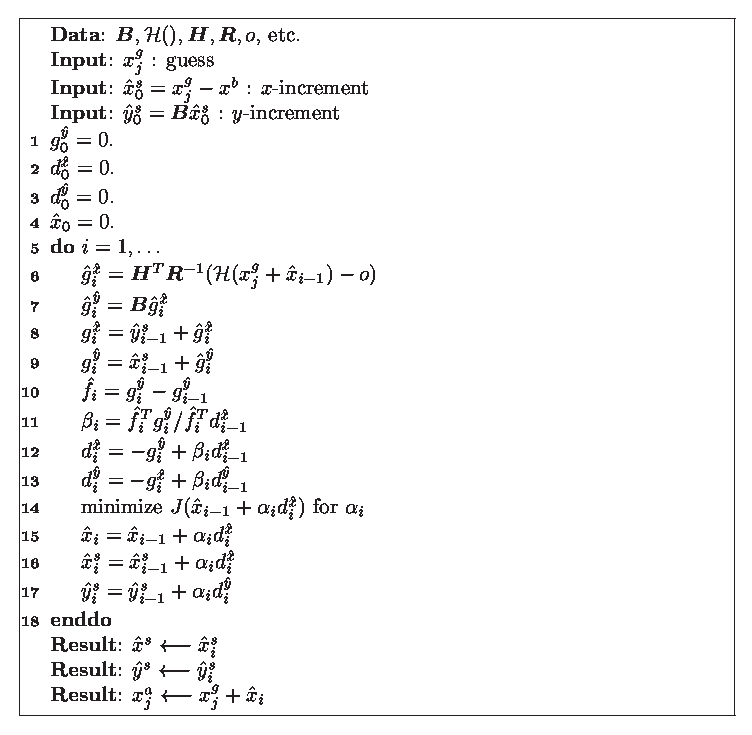
\includegraphics{algo-pcgsoi-math.eps}}

\caption{Routine {\tt PCGSOI()} in mathematical terms.}
\label{alg:algo}
\end{figure}

In Fig.~\ref{alg:algo},
the objective of code segment line 6-9 is to compute the gradient
with respect to $\xhat$ ({\em i.e.} $\xhatsave$) and $\yhatsave$,
respectively.  Line 10-13 is to compute the correction directions
in $\xhat$ ($\xhatsave$) and $\yhatsave$, where line 11 for
scalar $\beta$
is in agreement with Eqs.~(106) and (107) in Navon and Legler (1987),
in the ``one-step limited-memory BFGS quasi-Newton update'' form.
Line 14 is to compute the step-size
that minimize the cost function along the given correction direction
$\dirx_i$ or $\diry_i$, which
can also be noted as ``solve
\begin{align*}
0 &=(\dirx_i)^T\!\nabla_\xhat J	\\
  &=(\dirx_i)^T\!\yhatsave +
    (\dirx_i)^T\!\bH^T\Rinv
	\bigl(\cH(x_j^g+\xhat_{i-1}+\alpha_i\dirx_i)-o\bigr)	\\
  &=(\diry_i)^T\!\xhatsave +
    (\dirx_i)^T\!\bH^T\Rinv
	\bigl(\cH(x_j^g+\xhat_{i-1}+\alpha_i\dirx_i)-o\bigr)	\\
  &=(\diry_i)^T\!\nabla_\yhatsave J
\end{align*}
for $\alpha_i$''.
Line 15-17, is to compute the next values of $\xhat$ ($\xhatsave$)
and $\yhatsave$.

%\documentclass{article}
\usepackage{fancybox}
\usepackage{graphics}
\usepackage{color}
\usepackage{bm}
\usepackage{amssymb,amsmath}
\usepackage[
figure,
longend,
boxed,
linesnumbered,
noline
]{algorithm2e}
\begin{document}
\pagestyle{empty}
\newcommand{\tc}[2]{\textcolor{#1}{#2}}
\newcommand{\mc}[2]{{\color{#1}#2}}

\newcommand{\onehalf}{{\frac{1}{2}}}

\newcommand{\cH}{{\mathcal H}}
\newcommand{\cL}{{\mathcal L}}
\newcommand{\cM}{{\mathcal M}}

\newcommand{\bH}{\bm H}
\newcommand{\bP}{\bm B}
\newcommand{\bR}{\bm R}
\newcommand{\bB}{\bm B}
\newcommand{\Rinv}{{\bm R}^{-1}}
\newcommand{\bL}{\bm L}
\newcommand{\bM}{\bm M}

\newcommand{\xhat}{{\hat{x}}}
\newcommand{\yhat}{{\hat{y}}}

\newcommand{\dirx}{d^\xhat}
\newcommand{\diry}{d^\yhat}

\newcommand{\xhatsave}{{\xhat^s}}
\newcommand{\yhatsave}{{\yhat^s}}

\newcommand{\ghatx}{\hat{g}^\xhat}
\newcommand{\ghaty}{\hat{g}^\yhat}

\newcommand{\gradx}{g^\xhat}

\newcommand{\grady}{g^\yhat}

\newcommand{\fhat}{{\hat{f}}}

%\newcommand{\red}{\color{green}}
\newcommand{\red}{}



\SetKwComment{comm}{!}{}
\SetKwFor{Fdo}{do}{}{enddo}
\SetKwFor{Fwhile}{while}{do}{endwhile}
\SetKwFor{Fwhere}{where}{do}{endwhere}
\SetKwFor{Fforall}{forall}{do}{endforall}
\SetKwSwitch{Fselect}{Fcase}{Fother}{select}{}{case}{}{end select}
\dontprintsemicolon
\SetKw{default}{\rm default}



\begin{algorithm}[h]
\KwData{$\bB, \cH(), \bH, \bR, o$, etc.}	\;
\KwIn{$x^g$, $q^a$ : present guess/analysis in different grid spaces}						\;
\KwIn{$\xhatsave$ : $= x^g - {\bm L}^{-1}q^b$, $x$-increment}	\;
\KwIn{$\yhatsave$ : $= \bB \xhatsave$, $y$-increment}	\;

$\dirx = 0.$	\;
$\diry = 0.$	\;
$\xhat = 0.$	\;
$\fhat = 0.$	\;

\Fdo{$i=1,\ldots $}{
  $\gradx =
    {\bH^T \Rinv (\cH(x^g+{\red\xhat}) - o)}$	\;

  $\grady = {\bB \gradx}$				\;

  $\gradx = {\red \yhatsave} + \gradx$	\;
  $\grady = {\red \xhatsave} + \grady$	\;

  $\fhat = \grady - {\red \fhat}$		\;
  $\beta = {\fhat}^T\grady / {\fhat}^T{\red \dirx}$;
  $\fhat = \grady$	\;

  $\dirx = -\grady + \beta{\red \dirx}$	\;
  $\diry = -\gradx + \beta{\red \diry}$	\;

  minimize $J(\xhat+\alpha\dirx)$ for $\alpha$	\;
%  \{solve
%  	$0={\dirx}^T\!\bigl({\red\yhatsave}+\bH^T \Rinv (
%		\cH(x^g+{\red\xhat}+\alpha\dirx) - o )
%	\bigr)$ for $\alpha$\}		\;
  
  $\xhat = {\red \xhat} + \alpha \dirx$	\;
  $\xhatsave = {\red \xhatsave} + \alpha \dirx$	\;
  $\yhatsave = {\red \yhatsave} + \alpha \diry$	\;
}
$q^a = q^a+ {\bm L}\xhat $			\;
\KwResult{$\xhatsave, \yhatsave, q^a$}	\;
\end{algorithm}
\end{document}

\begin{figure}[hb]
\resizebox{!}{!}{
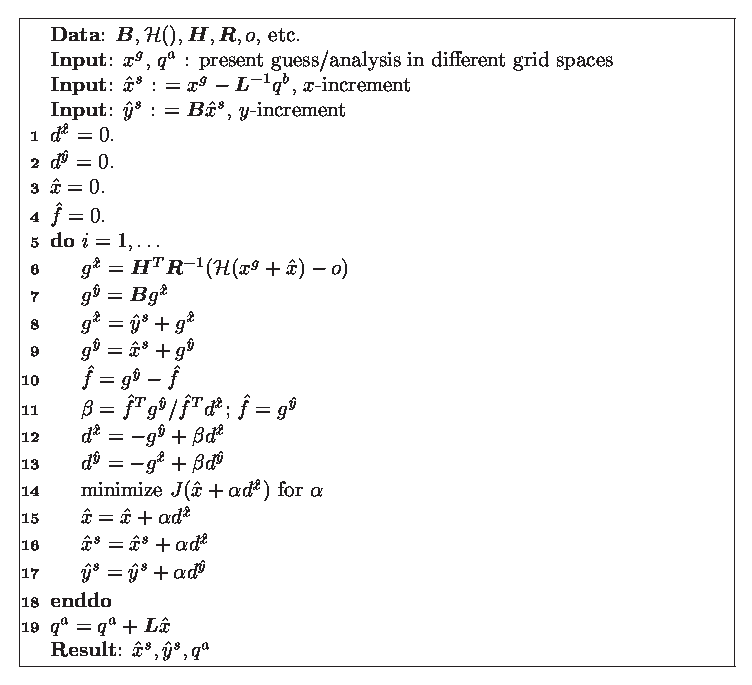
\includegraphics{algo-pcgsoi-code.eps}}

\caption{Routine {\tt PCGSOI()} in program terms.
Note two new operators ${\bm L}$ and ${\bm L}^{-1}$.
} \label{alg:code}
\end{figure}

The algorithm shown in Fig.~\ref{alg:algo} and Fig.~\ref{alg:code} is
known as the ``inner-loop'' of the minimization process in the GSI, or
\verb"SUBROUTINE PCGSOI()".  Note that beside that Fig.~\ref{alg:algo}
is in mathematical terms and Fig.~\ref{alg:code} is in program terms,
Fig.~\ref{alg:code} also identifies the difference between the source
grid-space defining background state $q^b$ and analysis $q^a$, and the
intermediate grid-space defining the guess state $x^g$ and the
increment state $\xhat$, and two linear operators
($\bL$ and $\bL^{-1}$) converting between
the two spaces back-and-forth.

The algorithm descriptions given in these two figures
include neither some configuration steps for the ``inner-loop'', nor
the so-called ``restart'' of the search directions.  Both are parts of
the algorithm known as the ``outer-loop'' of the process in the GSI,
or in \verb"SUBROUTINE GLBSOI()".

Figure~\ref{alg:twoloops} describes
the complete minimization process in its two level nested-loop form,
for the algorithm in routine \verb"GLBSOI()" as well as
its major lower level routines.
For convenience, some of these lower level
routines are marked as Fortran comments in the figure.
Note that the description of line 4-6 is highly simplified,
not an accurate representation of the complex details in this
part of the whole algorithm.

%\documentclass{article}
\usepackage{fancybox}
\usepackage{graphics}
\usepackage{color}
\usepackage{bm}
\usepackage{amssymb,amsmath}
\usepackage[
figure,
longend,
boxed,
linesnumbered,
noline
]{algorithm2e}
\begin{document}
\pagestyle{empty}
\newcommand{\tc}[2]{\textcolor{#1}{#2}}
\newcommand{\mc}[2]{{\color{#1}#2}}

\newcommand{\onehalf}{{\frac{1}{2}}}

\newcommand{\cH}{{\mathcal H}}
\newcommand{\cL}{{\mathcal L}}
\newcommand{\cM}{{\mathcal M}}

\newcommand{\bH}{\bm H}
\newcommand{\bP}{\bm B}
\newcommand{\bR}{\bm R}
\newcommand{\bB}{\bm B}
\newcommand{\Rinv}{{\bm R}^{-1}}
\newcommand{\bL}{\bm L}
\newcommand{\bM}{\bm M}

\newcommand{\xhat}{{\hat{x}}}
\newcommand{\yhat}{{\hat{y}}}

\newcommand{\dirx}{d^\xhat}
\newcommand{\diry}{d^\yhat}

\newcommand{\xhatsave}{{\xhat^s}}
\newcommand{\yhatsave}{{\yhat^s}}

\newcommand{\ghatx}{\hat{g}^\xhat}
\newcommand{\ghaty}{\hat{g}^\yhat}

\newcommand{\gradx}{g^\xhat}

\newcommand{\grady}{g^\yhat}

\newcommand{\fhat}{{\hat{f}}}

%\newcommand{\red}{\color{green}}
\newcommand{\red}{}



\SetKwComment{comm}{!}{}
\SetKwFor{Fdo}{do}{}{enddo}
\SetKwFor{Fwhile}{while}{do}{endwhile}
\SetKwFor{Fwhere}{where}{do}{endwhere}
\SetKwFor{Fforall}{forall}{do}{endforall}
\SetKwSwitch{Fselect}{Fcase}{Fother}{select}{}{case}{}{end select}
\dontprintsemicolon
\SetKw{default}{\rm default}



\begin{algorithm}[h]

$\xhatsave = 0.$		\;
$\yhatsave = 0.$		\;
\Fdo{$j=1,\ldots $}{
  $q^a \longleftarrow \text{input } q^b$ if {\em j.eq.1}; and
	$x^g = {\bm L}^{-1}q^a$
	\comm{ {\tt read\_guess()}}	\;

  setup for $\bB \xhat$ operation if {\em j.eq.1}
	\comm{ \tt prewgt()}
	\;

  setup for $\bH^T \Rinv (\cH(x^g+\xhat)-o)$ operation
	\comm{ {\tt setuprhsall()}}
	\;

$\dirx = 0.$	\;
$\diry = 0.$	\;
$\xhat = 0.$	\;
$\fhat = 0.$	\;

\Fdo{$i=1,\ldots $}{
  $\gradx =
	{\bH^T \Rinv (\cH(x^g+{\red\xhat}) - o)}$
	\comm{ \tt intall()}
	\;

  $\grady = {\bB \gradx}$
	\comm{ \tt berror()}
	\;

  $\gradx = {\red \yhatsave} + \gradx$	\;
  $\grady = {\red \xhatsave} + \grady$	\;

  $\fhat = \grady - {\red \fhat}$		\;
  $\beta = {\fhat}^T\!\grady / {\fhat}^T\!{\red \dirx}$;
  $\fhat = \grady$	\;

  $\dirx = -\grady + \beta{\red \dirx}$	\;
  $\diry = -\gradx + \beta{\red \diry}$	\;

  minimize $J(\xhat+\alpha\dirx)$ for $\alpha$
	\comm{ \tt stpcalc()}
	\;
%  \{solve
%  	$0={\dirx}^T\!\bigl({\red\yhatsave}+\bH^T \Rinv (
%		\cH(x^g+{\red\xhat}+\alpha\dirx) - o )
%	\bigr)$ for $\alpha$\}		\;
  
  $\xhat = {\red \xhat} + \alpha \dirx$	\;
  $\xhatsave = {\red \xhatsave} + \alpha \dirx$	\;
  $\yhatsave = {\red \yhatsave} + \alpha \diry$	\;
}
$q^a = q^a+ {\bm L}\xhat $	
	\comm{ \tt hopers()}
	\;
}
write out $q^a$
	\comm{ \tt write\_all()}
	\;
\end{algorithm}

\end{document}

\begin{figure}[hb]
\resizebox{!}{!}{
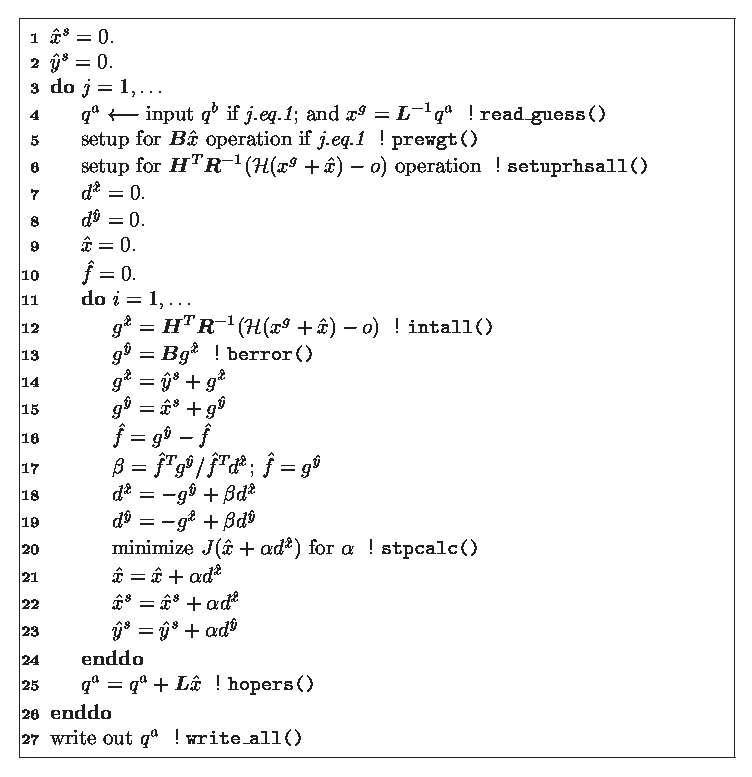
\includegraphics{algo-glbsoi-code.eps}}
\caption{Minimization in two level nested loops
from routine {\tt GLBSOI()} down.
} \label{alg:twoloops}
\end{figure}

\end{document}
